%%%%%%%%%%%%%%%%%%%%%%%%%%%%%%%%%%%%%%%%%%%%%%%%%%%%%%%%%%%%%%%%%%%%%%%%%%%%%%
% A user guide for semtex spectral element code.
%
% $Id$
%%%%%%%%%%%%%%%%%%%%%%%%%%%%%%%%%%%%%%%%%%%%%%%%%%%%%%%%%%%%%%%%%%%%%%%%%%%%%%
\documentclass[11pt,a4paper]{report}

\usepackage{graphicx}
\usepackage{natbib}
\usepackage{bm}

\graphicspath{{./Figs/}}

\setlength{\textheight}              {245mm}
\setlength{\textwidth}               {160mm}
\setlength{\topmargin}               {-20mm}
\setlength{\oddsidemargin}           {0mm}
\setlength{\parindent}               {2.5ex}
\setlength{\leftmargin}              {2.5ex}
\setlength{\bibsep}                  {\parskip}

\renewcommand{\baselinestretch}      {1.0}
\renewcommand{\familydefault}{cmss}

\def\bs#1{\mbox{\boldmath$#1$}}                     % bold symbol typeface
\def\vec#1{\mbox{\bf#1}}                            % bold vector typeface
\def\Rey{\mbox{\it Re}}                             % Reynolds number
\def\St{\mbox{\it St}}                              % Strouhal number
\def\undertext#1{$\underline{\smash{\hbox{#1}}}$}   % underline running text
\def\refitem{\noindent\hangindent=2em}              % hanging index for refs.

%%%%%%%%%%%%%%%%%%%%%%%%%%%%%%%%%%%%%%%%%%%%%%%%%%%%%%%%%%%%%%%%%%%%%%%%%%%%%%
\begin{document}

\begin{titlepage}
\centering

\vspace*{\fill}

{\huge Using {\sffamily semtex}}

\vspace{\fill}

\begin{figure}[h]
\begin{center}
\fbox{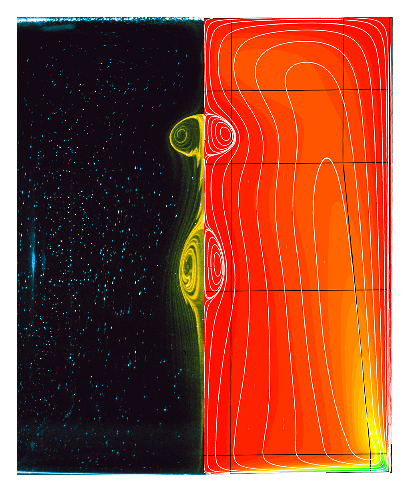
\includegraphics[width=0.5\textwidth]{vbmed_bitmap.eps}}
\end{center}
\end{figure}

\vspace{\fill}

{\large H.\,M. Blackburn}\\
CSIRO Manufacturing and Materials Technology\\

\vspace{\fill}

{\large CSIRO Doc.\ 97/159(M)}\\
\today

\textsf{semtex} version 6.1

\vspace*{\fill}

\end{titlepage}

%%%%%%%%%%%%%%%%%%%%%%%%%%%%%%%%%%%%%%%%%%%%%%%%%%%%%%%%%%%%%%%%%%%%%%%%%%%%%%

\tableofcontents

\clearpage

%%%%%%%%%%%%%%%%%%%%%%%%%%%%%%%%%%%%%%%%%%%%%%%%%%%%%%%%%%%%%%%%%%%%%%%%%%%%%
\chapter{Introduction}

\textsf{Semtex} is a family of spectral element simulation codes.  The
spectral element method is a high-order finite element technique that
combines the geometric flexibility of finite elements with the high
accuracy of spectral methods.  The method was pioneered in the mid
1980's by Anthony Patera at MIT \cite{pat84,kp86}. \textsf{Semtex}
uses parametrically mapped quadrilateral elements, and the `nodal'
shape function basis.

%-----------------------------------------------------------------------------
\section{Numerical method}

Some central features of the spectral element method are
\begin{description}
\item[Orthogonal polynomial-based shape functions] Spectral accuracy
is achieved by using tensor-product Lagrange interpolants within each
element, where the nodes of these shape functions are placed at the
zeros of Legendre polynomials mapped from the canonical domain
[-1,~1]$\times$[-1,~1] to each element.  In one spatial dimension, the
resulting Gauss--Lobatto--Legendre Lagrange interpolant which is~1 at
one of the $N + 1$ Gauss--Lobatto points $x_j$ in [-1, 1] and~0 at the
others is
\begin{equation}
\psi_j(x) = \frac{1}{N(N+1)L_N(x_j)}\frac{(1-x^2)L_N^\prime(x)}{x - x_j}.
\end{equation}
For example, the family of sixth-order GLL Lagrange interpolants is
shown in figure~\ref{fig:shapes}.
\begin{figure}

\begin{center}
  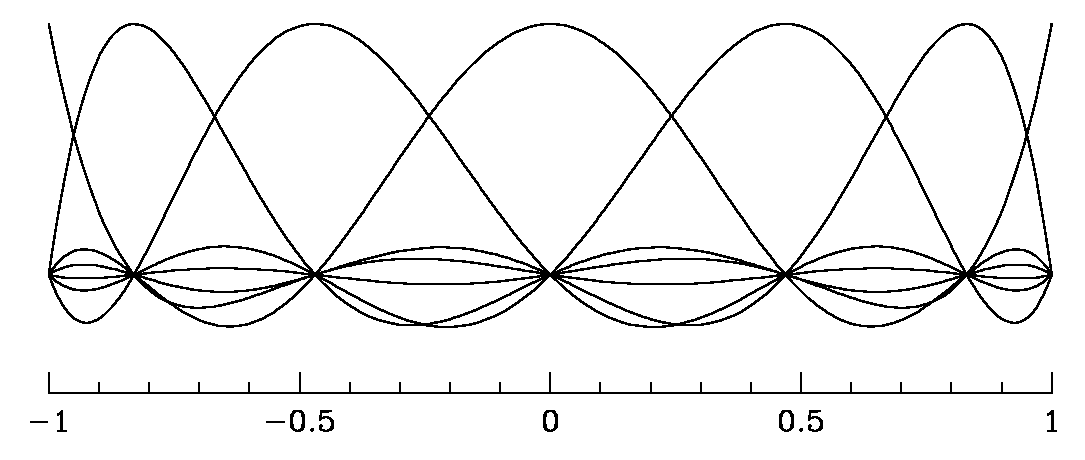
\includegraphics[width=0.5\textwidth]{shape7x7.eps}
\end{center}
\caption{The family of sixth-order one-dimensional GLL Lagrange shape
  functions on the master domain $[-1,+1]$.}
\label{fig:shapes}
\end{figure}
In smooth function spaces it can be shown that the resulting
interpolants converge exponentially fast (faster than any negative
integer power of $N$) as the order of the interpolant is increased.
See \citet{chqz88}, \S\S\,2.3.2 and~9.4.3.
\item[Gauss--Lobatto quadrature]
Efficiency (particularly in iterative methods) is achieved by
using Gauss--Lobatto quadrature for evaluating elemental integrals: the
quadrature points reside at the nodal points, which enables fast
tensor-product techniques to be used for iterative matrix solution
methods.  Gauss--Lobatto quadrature delivers diagonal mass matrices.
\item[Static condensation]
Direct matrix solutions are sped up by using static condensation
coupled with bandwidth reduction algorithms to reduce storage
requirements for assembled system matrices.
\end{description}

While the numerical method is very accurate and efficient, it also has
the advantage that complex geometries can be accommodated by employing
unstructured meshes.  The vertices of spectral elements meshes can be
produced using finite-element mesh generation procedures.

%-----------------------------------------------------------------------------
\section{Implementation}

The top level of the code is written in C++, with calls to C and
FORTRAN library routines, e.g.\ BLAS \& LAPACK. The original
implementation for two-dimensional Cartesian geometries was extended
to three dimensions using Fourier expansion functions for
spatially-periodic directions in Cartesian and cylindrical spaces.
Concurrent execution is supported, using MPI as the basis for
interprocessor communications, and the code has been ported to DEC,
NEC, Fujitsu, Compaq, SGI, Apple and Linux multiprocessor
machines. Basically it ought to work with little trouble on any
contemporary UNIX system.

There are various code extensions that are not part of the base
distribution. These include dynamic and non-dynamic LES
\citep{blsc03}, simple power-law type non-Newtonian rheologies
\citep{rb06}, scalar transport \citep{hmb01a,hmb02b}, buoyancy via the
Boussinesq approximation, accelerating frame of reference coupling for
aeroelasticity \citep{bh96a,bh99,bgw01,hmb03}, solution of
steady-state flows via Newton-Raphson iteration \citep{hmb02a}, linear
stability analysis
\citep{hmb02a,bllo03b,bllo03a,bml04,shbl04,ebs06,blsh06}.

%-----------------------------------------------------------------------------
\section{Further reading}

The most comprehensive references on spectral methods in general are
\citet{gs77} and \citet{chqz88}.  The first papers by \citet{pat84}
and \citet{kp86} provide a good introduction to spectral elements,
although some aspects have changed with time and \citet{mt89} is more
up-to-date.  The use of Fourier expansions to extend the method to
three spatial dimensions is discussed by \citet{ap89}, \citet{kar89}
and \citet{kar90}.  The use of spectral element techniques in
cylindrical coordinates is dealt with in \citet{blsh04}.  The
time-splitting method used for time integration is described by
\citet*{kio91}.  The book by \citet{fun97} provides useful information
and further references.  Recent overviews and some applications appear
in \citet{kh98,hen99b}.  The definitive reference is now the book by
\citet{kars05}, but you may also find the text by \citet*{dfm02}
useful for alternative explanations and views.

%%%%%%%%%%%%%%%%%%%%%%%%%%%%%%%%%%%%%%%%%%%%%%%%%%%%%%%%%%%%%%%%%%%%%%%%%%%%%
\chapter{Starting out}

It is assumed you're using some version of UNIX, and the current
versions assume that your C++ compiler supports the standard
libraries. Makefiles assume GNUmake.  SuperMongo and TECPLOT would be
nice to have but are not essential to get up and running.  All major
executables have a \texttt{-h} command line option which provides a
usage prompt.

Application programs/Makefiles can be found in top and upper-level
directories:
\begin{tabbing}
\texttt{elliptic}    \= 
        Solve elliptic (Laplace, Poisson, Helmholtz) problems.\\
\texttt{dns} \>
        Solve time-varying Navier--Stokes problems, Cartesian/cylindrical.\\
\end{tabbing}
The Navier--Stokes solver can also be used to solve unsteady Stokes
problems.

%============================================================================
\section{Testing}

Unpack the tar file, then run \texttt{make test}. This will copy
header files to their correct places, compile and place the libraries,
make two central utilities (\texttt{compare} and \texttt{enumerate}),
then make the direct numerical simulation solver \texttt{dns} and run
regression checks on its output for a number of test cases. If all
goes well, this process will end with a number of tests reported as
\texttt{passed}. 

%----------------------------------------------------------------------------
\subsection{Troubleshooting}
If the above process didn't work, there are a number of possible
things lacking on your system, e.g.:
\begin{enumerate}
\item
GNU's \texttt{make}: it needs to be in your
\texttt{path} somewhere under the name \texttt{gmake}.
\item
the BLAS and LAPACK libraries\,---\,these should be
either under \texttt{/usr/lib} or in \texttt{/usr/local/lib}: search
for \texttt{libblas} and \texttt{liblapack}.
\item
a standard C++ compiler, or a FORTRAN77 compiler.
\end{enumerate}
As well, check the \texttt{README} file in the top directory. Of
course, it is possible that the code is incompatible with some detail
of your compilation system or has a bug, but it has had fairly
extensive exercise on a number of UNIX systems by now.


%============================================================================
\section{Files}

\textsf{Semtex} uses a base input file which describes the mesh,
boundary conditions.  We call this a \verb+session+ file and
typically it has no root extension.  It is written in a format
patterned on HTML, which we have called FEML (for Finite Element
Markup Language).  There are a number of example session files in the
mesh directory.  Other files have standard extensions:
\begin{tabbing}
\texttt{session.num}  \=
        Global node numbers, produced by enumerate utility.\\
\texttt{session.fld}  \>
        Solution/field file.  Binary format by default.\\
\texttt{session.rst}  \>
        Restart file. Read in to initialize solution if present.\\
\texttt{session.avg} \> Averaged results. Read back in for
        continuation (over-written).\\
\texttt{session.his} \> History point data.\\
\texttt{session.flx} \> Time series of pressure and viscous forces
        integrated over the \texttt{wall} boundary group.\\
\texttt{session.mdl} \> Time series of kinetic energies in the Fourier
        modes (only for 3D execution).\\
\texttt{session.par} \> Used to define initial particle locations.\\
\texttt{session.trk} \> Integrated particle locations.\\
\end{tabbing}

When writing a new session file it is best to run \texttt{meshpr}
(and/or \texttt{meshpr -c}) on it before trying to use it for
simulations.  \texttt{Meshpr} will catch most of the easier-to-make
errors.  You can also plot up the results using SuperMongo or other
utility as a visual check.

%============================================================================
\section{Utilities}

Source code for these is found in the \texttt{utility} directory. You
will need to make most of these by hand (using the supplied
\texttt{Makefile}).  Here is a summary:
\begin{tabbing}
\texttt{enumerate}  \= \kill
\texttt{addfield} \>   
        Add vorticity vector components, divergence, etc., to a field
	file.\\
\texttt{calc} \>      
        A simple calculator that calls \verb+femlib+'s function
        parser. The default functions\\\>and \texttt{TOKENS} can be seen
        if you run \texttt{calc -h}.\\
\texttt{compare} \>   
        Generate restart files, compare solutions to a function.\\
\texttt{convert} \>   
        Convert field file formats (IEEE-big/little, ASCII).\\
\texttt{eneq} \>   
        Compute terms in the energy transport equation.\\
\texttt{enumerate}  \>
        Generate global node numbering, with RCM optimization.\\
\texttt{integral} \> Obtain the 2D integral of fields over the
        domain area.\\
\texttt{interp} \>   
        Interpolate a field file onto a (2D) set of points.\\
\texttt{meshpr} \>    
        Generate 2D mesh locations for plotting or checking.\\
\texttt{noiz} \>      
        Add a random perturbation to a field file.\\
\texttt{probe} \>   
        Probe a field file at a set of 2D/3D points. Different
        interfaces to \texttt{probe}\\ \> are obtained through the names
        \texttt{probeline} and \texttt{probeplane}: \\ \> make these soft
        links by hand.\\
\texttt{project} \>   
        Convert a field file to a different order interpolation.\\
\texttt{rectmesh} \>
        Generate a template session file for a rectangular domain.\\
\texttt{resubmit} \> Shell utility for automatic job resubmission.\\
\texttt{rstress} \>
	Postprocess to compute Reyolds stresses from a file of
        time-averaged variables.\\
\texttt{save} \> Shell utility for automatic job resubmssion.\\
\texttt{sem2tec} \>   
        Convert field files to Amtec TECPLOT format.\\
\texttt{transform} \>      
        Take Fourier, Legendre, modal basis transform of a field
	file. Invertible.\\
\texttt{wallmesh} \>      
        Extract the mesh nodes corresponding to surfaces with the
	\verb+wall+ group.
\end{tabbing}


%%%%%%%%%%%%%%%%%%%%%%%%%%%%%%%%%%%%%%%%%%%%%%%%%%%%%%%%%%%%%%%%%%%%%%%%%%%%%
\chapter{Examples}

We will run through some examples to illustrate input files, utility
routines, and the use of the solvers.

%============================================================================
\section{2D Taylor flow}

Taylor flow is an analytical solution to the Navier--Stokes equations.
In the $x$--$y$ plane the solution is 
\begin{eqnarray}
        u &=& -\cos(\pi x) \sin(\pi y) \exp(-2\pi^2\nu t),\\
        v &=& +\sin(\pi x) \cos(\pi y) \exp(-2\pi^2\nu t),\\
        p &=& -(\cos(2\pi x) + \cos(2\pi y)) \exp(-4\pi^2\nu t)/4.
\end{eqnarray}
The solution is doubly periodic in space, with periodic length 2.  As
usual for Navier--Stokes solutions, the pressure can only be specified
up to an arbitrary constant.  An interesting feature of this solution
is that the nonlinear and pressure gradient terms balance one another,
leaving a diffusive decay of the initial condition --- this property
is occasionally useful for checking codes.

%----------------------------------------------------------------------------
\subsection{Session file}

Below is the complete input or \textsl{session} file we will use; it
has four elements, each of the same size, with 11 nodes along each
edge.  We will call this session file \texttt{taylor2} in the
following.

{\small
\begin{verbatim}
##############################################################################
# 2D Taylor flow in the x--y plane has the exact solution
#
#       u = -cos(PI*x)*sin(PI*y)*exp(-2.0*PI*PI*KINVIS*t)
#       v =  sin(PI*x)*cos(PI*y)*exp(-2.0*PI*PI*KINVIS*t)
#       w =  0
#       p = -0.25*(cos(2.0*PI*x)+cos(2.0*PI*y))*exp(-4.0*PI*PI*KINVIS*t)
#
# Use periodic boundaries (no BCs).

<USER>
        u = -cos(PI*x)*sin(PI*y)*exp(-2.0*PI*PI*KINVIS*t)
        v =  sin(PI*x)*cos(PI*y)*exp(-2.0*PI*PI*KINVIS*t)
        p = -0.25*(cos(TWOPI*x)+cos(TWOPI*y))*exp(-4.0*PI*PI*KINVIS*t)
</USER>

<FIELDS>
        u v p
</FIELDS>

<TOKENS>
        N_TIME  = 2
        N_P     = 11
        N_STEP  = 20
        D_T     = 0.02
        Re      = 100.0
        KINVIS  = 1.0/Re
        TOL_REL = 1e-12
</TOKENS>

<NODES NUMBER=9>
        1       0.0       0.0       0.0
        2       1.0       0.0       0.0
        3       2.0       0.0       0.0
        4       0.0       1.0       0.0
        5       1.0       1.0       0.0
        6       2.0       1.0       0.0
        7       0.0       2.0       0.0
        8       1.0       2.0       0.0
        9       2.0       2.0       0.0
</NODES>

<ELEMENTS NUMBER=4>
        1 <Q> 1 2 5 4 </Q>
        2 <Q> 2 3 6 5 </Q>
        3 <Q> 4 5 8 7 </Q>
        4 <Q> 5 6 9 8 </Q>
</ELEMENTS>

<SURFACES NUMBER=4>
        1       1       1       <P>     3       3       </P>
        2       2       1       <P>     4       3       </P>
        3       2       2       <P>     1       4       </P>
        4       4       2       <P>     3       4       </P>
</SURFACES>
\end{verbatim}
}

The first section of the file in this case contains comments; a line
anywhere in the session file which starts with a \verb+#+ is
considered to be a comment.  Following that are a number of sections
which are opened and closed with matching keywords in HTML style (e.g.
\verb+<USER>+--\verb+<\USER>+).  Keywords are not case sensitive.
The complete list of keywords is: \texttt{TOKENS}, \texttt{FIELDS}, 
\texttt{GROUPS}, \texttt{BCS}, \texttt{NODES}, \texttt{ELEMENTS}, 
\texttt{SURFACES}, \texttt{CURVES} and \texttt{USER}.  Depending on the
problem being solved, some sections may not be needed, but the minimal
set is: \texttt{FIELDS}, \texttt{NODES}, \texttt{ELEMENTS} and
\texttt{SURFACES}.  Anywhere there is likely to be a long list of
inputs within the sections, the \texttt{NUMBER} of inputs is also
required; this currently applies to \texttt{GROUPS}, \texttt{BCS},
\texttt{NODES}, \texttt{ELEMENTS}, \texttt{SURFACES} and
\texttt{CURVES}.  In each of these cases the numeric tag appears first for
each input, which is free-format.  The order in which the sections
appear in the session file is irrelevant.

The \texttt{USER} section is ignored by the solvers, and is used
instead by utilities --- in this case it will be used by the
\texttt{compare} utility both to generate the initial condition or
\textsl{restart} file and to check the computed solution.  This
section declares the variables corresponding to the solution fields
with the corresponding analytical solutions.  The variables
\texttt{x}, \texttt{y}, \texttt{z} and \texttt{t} can be used to
represent the three spatial coordinates and time.  Note that some
constants such as \texttt{PI} and \texttt{TWOPI} are predefined, while
others, like \texttt{KINVIS}, are set in the \texttt{TOKENS} section.
Note also the use of predefined functions, accessed through an inbuilt
function parser\footnote{The built-in functions and predefined constants
can be found by running \texttt{calc -h}.}.

The \texttt{FIELDS} section declares the one-character names of
solution fields.  The names are significant: \texttt{u}, \texttt{v}
and \texttt{w} are the three velocity components (we only use
\texttt{u} and \texttt{v} here for a 2D solution and the \texttt{w}
component is always the direction of Fourier expansions), \texttt{p}
is the pressure field.  The field name \texttt{c} is also recognized
as a scalar field for certain solvers, e.g. the elliptic solver.

In the \texttt{TOKENS} section, second-order accurate time integration
is selected (\verb+N_TIME = 2+) and the number of Lagrange knot points
along the side of each element is set to 11 (\verb+N_P = 11+).  The
code will integrate for 20 timesteps (\verb+N_STEP = 20+) with a
timestep of 0.02 (\verb+D_T = 0.002+).  The kinematic viscosity is
set as the inverse of the Reynolds number (100): note the use of the
function parser here.  Finally the relative tolerance used as a
stopping test in the PCG iteration used to solve the viscous substep
on the first timestep is set as $1.0\times10^{-12}$.

The shape of the mesh is defined by the \texttt{NODES} and
\texttt{ELEMENTS} sections.  Here there are four elements, each
obtained by connecting the corner nodes in a counterclockwise
traverse.  The $x$, $y$ and $z$ locations of the nodes are given, and
the four numbers given for the nodes of each element are indices
within the list of nodes.

In the final section (\texttt{SURFACES}), we describe how the edges of
elements which define the boundary of the solution domain are dealt
with.  In this example, the solution domain is periodic and there are
no boundary conditions to be applied, so the \texttt{SURFACES} section
describes only periodic (\verb+P+) connections between elements.  For
example, on the first line, side~1 of element~1 is declared to be
periodic with side~3 of element~3 --- side~1 runs between the first
and second nodes, while side~3 runs between the third and fourth.

%----------------------------------------------------------------------------
\subsection{Running the codes}

Assume we're in the \texttt{dns} directory of the distribution, that
the \texttt{enumerate}, \texttt{compare}, \texttt{meshpr} and
\texttt{sem2tec} utilities have been compiled, as well as the
\texttt{dns} simulation code.
{\small
\begin{verbatim}
karman[16] cp ../mesh/taylor2 .
\end{verbatim}
}

First we'll examine the mesh, using SuperMongo macros.
{\small
\begin{verbatim}
karman[17] meshpr taylor2 > taylor2.msh
karman[18] sm
Hello Hugh, please give me a command
: meshplot taylor2.msh 1
Read lines 1 to 1 from taylor2.msh
Read lines 2 to 485 from taylor2.msh
: meshnum
: meshbox
: quit
\end{verbatim}
}
\noindent
You should have seen a plot like that in figure~\ref{tay2msh}. (Note:
while you are building up the mesh parts of a session file, you can
use \texttt{meshpr -c} to suppress some of the checking for matching
element edges and curved boundaries that \texttt{meshpr} does by
default.)
\begin{figure}
\begin{center}
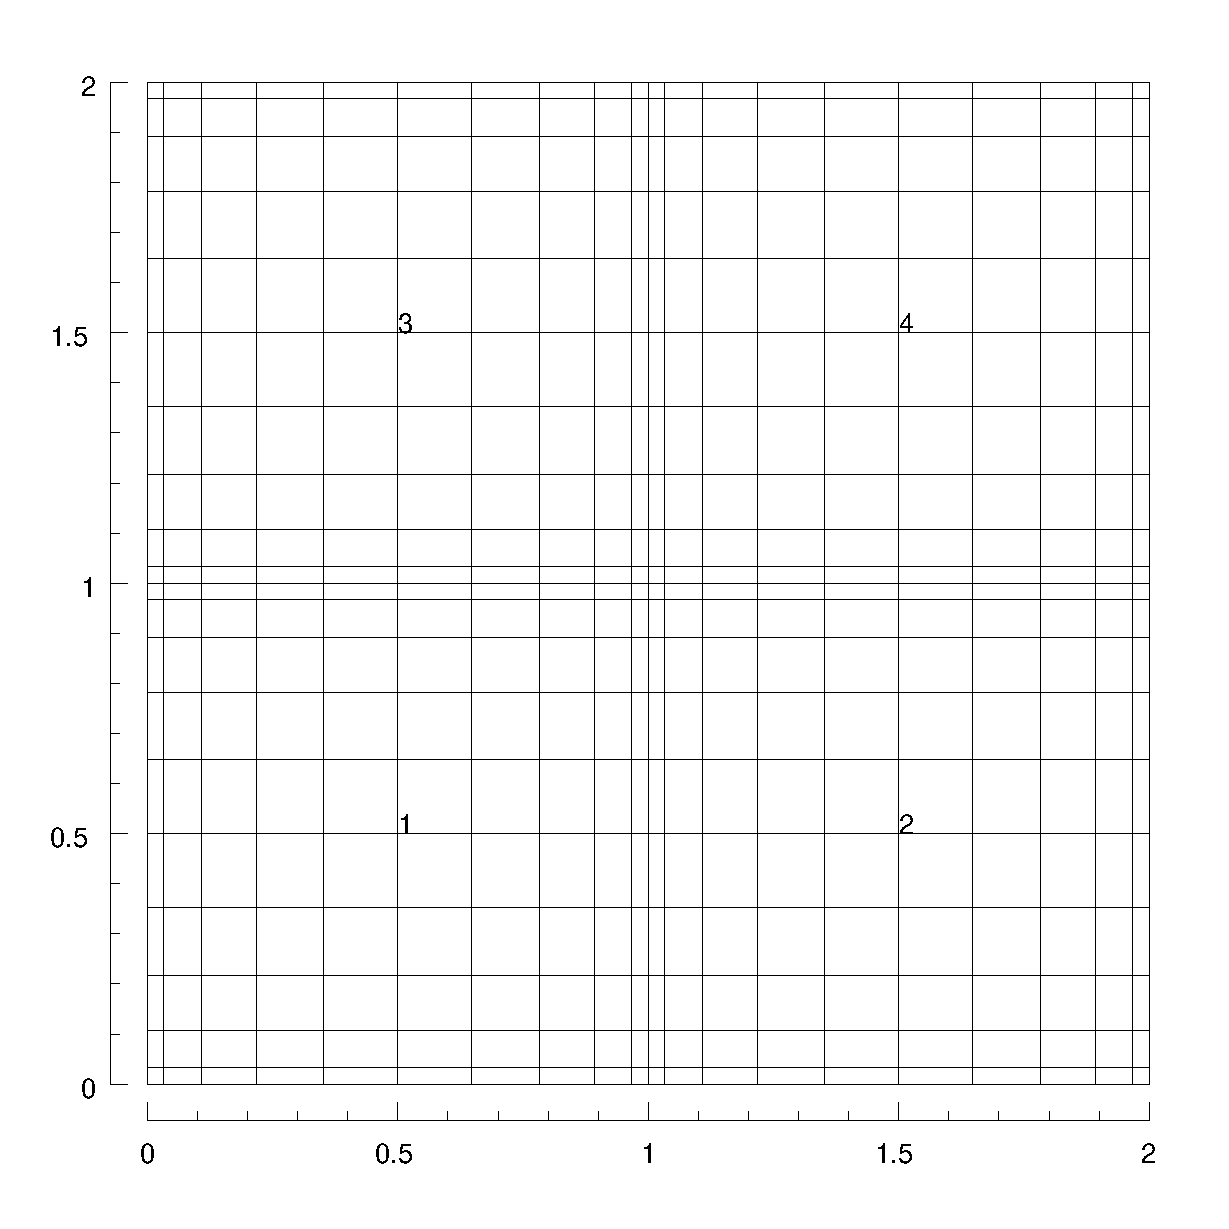
\includegraphics[width=0.5\textwidth]{taylor2mesh.eps}
\end{center}
\caption{
\label{tay2msh}
  The mesh corresponding to the \texttt{taylor2} session file.
}
\end{figure}

Next we will generate the global numbering schemes for the solution
using \texttt{enumerate} to produce \texttt{taylor2.num}.  The
solution code would run \texttt{enumerate} automatically to generate
\texttt{taylor2.num} if it were not present, but we will run it `by
hand' to highlight its existence and illustrate its use.
{\small
\begin{verbatim}
karman[19] enumerate taylor2 > taylor2.num
karman[20] head -20 taylor2.num
# FIELDS         :  uvp
# ----------------  ----------
# 1 NUMBER SETS  :         uvp
# NEL            :           4
# NP_MAX         :          11
# NEXT_MAX       :          40
# NINT_MAX       :          81
# NTOTAL         :         484
# NBOUNDARY      :         160
# NGLOBAL        :          76
# NSOLVE         :          76
# OPTIMIZATION   :           1
# BANDWIDTH      :          67
# ----------------  ----------
# elmt  side offst  bmap  mask
     1     1     0    20     0
     1     1     1    17     0
     1     1     2    16     0
     1     1     3    15     0
     1     1     4    14     0
\end{verbatim}
}

The \texttt{compare} utility is used to generate a file of initial
conditions.  This \textsl{restart} file contains binary data, but
we'll have a look at the start of it by converting it to ASCII format.
Also, the header of these files is always in ASCII format, and so can
be examined directly using the Unix \texttt{head} command.
{\small
\begin{verbatim}
karman[21] compare taylor2 > taylor2.rst
karman[22] convert taylor2.rst | head -20
taylor2                   Session
Wed Aug 13 21:39:47 1997  Created
11   11   1    4          Nr, Ns, Nz, Elements
0                         Step
0                         Time
0.02                      Time step
0.01                      Kinvis
1                         Beta
uvp                       Fields written
ASCII                     Format
     0.000000000      0.000000000    -0.5000000000 
     0.000000000     0.1034847104    -0.4946454574 
     0.000000000     0.3321033052    -0.4448536974 
     0.000000000     0.6310660897    -0.3008777952 
     0.000000000     0.8940117093    -0.1003715318 
     0.000000000      1.000000000      0.000000000 
     0.000000000     0.8940117093    -0.1003715318 
     0.000000000     0.6310660897    -0.3008777952 
     0.000000000     0.3321033052    -0.4448536974 
     0.000000000     0.1034847104    -0.4946454574 
\end{verbatim}
}

Then the \texttt{dns} solver is run to generate a solution or
\textsl{field} file, \texttt{taylor2.fld}.  This has the same format
as the restart file.
{\small
\begin{verbatim}
karman[23] dns taylor2
-- Restarting from file:  taylor2.rst
   Start time       : 0
   Time step        : 0.02
   Number of steps  : 20
   End time         : 0.4
   Integration order: 2
-- Building matrices for Fields "uvp"   [*]
-- Building matrices for Fields "uvp"   [.]
-- Building matrices for Fields "uvp"   [*]
Step: 1  Time: 0.02
Step: 2  Time: 0.04
Step: 3  Time: 0.06
Step: 4  Time: 0.08
Step: 5  Time: 0.1
Step: 6  Time: 0.12
Step: 7  Time: 0.14
Step: 8  Time: 0.16
Step: 9  Time: 0.18
Step: 10  Time: 0.2
Step: 11  Time: 0.22
Step: 12  Time: 0.24
Step: 13  Time: 0.26
Step: 14  Time: 0.28
Step: 15  Time: 0.3
Step: 16  Time: 0.32
Step: 17  Time: 0.34
Step: 18  Time: 0.36
Step: 19  Time: 0.38
Step: 20  Time: 0.4
\end{verbatim}
}

We can use \texttt{compare} to examine how close the solution is to the
analytical solution.  The output of \texttt{compare} in this case
is a field file which contains the difference: since we're only interested
in seeing error norms here, we'll discard this field file.
{\small
\begin{verbatim}
karman[24] compare taylor2 taylor2.fld > /dev/null
Field 'u': norm_inf: 1.13019e-05
Field 'v': norm_inf: 1.13019e-05
Field 'p': norm_inf: 0.422391
\end{verbatim}
}
\noindent
The velocity error norms are small, as expected, but the pressure norm
will always be arbitrary, corresponding to the fact that the pressure
can only be specified to within an arbitrary constant.

Finally we will use \texttt{sem2tec} to generate a TECPLOT input file.
The TECPLOT utility \texttt{preplot} must also be in your \texttt{path}.
{\small
\begin{verbatim}
karman[36] sem2tec -m taylor2.msh taylor2.fld
\end{verbatim}
}
\noindent
This produces \texttt{taylor2.plt} which can be used as input to
\texttt{tecplot}.  The plot in figure~\ref{tay2soln} was generated
using \texttt{tecplot} and shows pressure contours and velocity
vectors.  Notice that by default \texttt{sem2tec} interpolates the
results from the Gauss--Lobatto--Legendre grid (seen in
figure~\ref{tay2msh}) used in the computation to a uniformly-spaced
grid of the same order.
\begin{figure}
\begin{center}
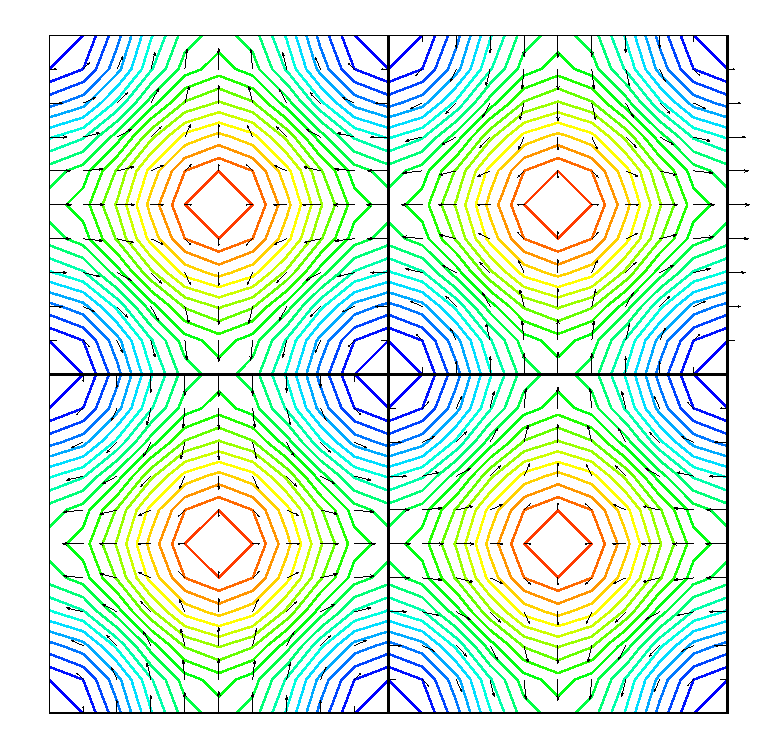
\includegraphics[width=0.5\textwidth]{taylor2.eps}
\end{center}
\caption{
\label{tay2soln}
  Solution to the \texttt{taylor2} problem, visualized using TECPLOT.
}
\end{figure}

%============================================================================
\section{2D Laplace problem}

In this section we illustrate the use of the elliptic solver for a 2D
Laplace problem, $\nabla^2 c = 0$.  In this case the function
\begin{equation}
  c(x,y) = \sin(x) \exp(-y)
\end{equation}
satisfies Laplace's equation and is used to set the boundary
conditions.  This example illustrates the methods used to set BCs and
also to generate curved element boundaries.  Also we will demonstrate
the selection of the PCG solver.  We will call the session file
\texttt{laplace6}.

The elliptic solver can also be used to solve Poisson and Helmholtz
problems in 2D and 3D Cartesian and cylindrical coordinate systems.
Apart from this use it provides a means to test new formulations of
elliptic solution routines used also in the Navier--Stokes type
solvers.

{\small
\begin{verbatim}
##############################################################################
# Laplace problem on unit square, BC c(x, y) = sin(x)*exp(-y)
# is also the analytical solution.  Use essential (Dirichlet) BC
# on upper, curved edge, with natural (Neumann) BCs elsewhere.

<FIELDS>
        c
</FIELDS>

<USER>
        c =  sin(x)*exp(-y)
</USER>

<TOKENS>
        N_P      = 11
        TOL_REL  = 1e-12
        STEP_MAX = 1000
</TOKENS>

<GROUPS NUMBER=4>
        1       d       value
        2       a       slope
        3       b       slope
        4       c       slope
</GROUPS>

<BCS NUMBER=4>
        1       d       1
                        <D>     c =  sin(x)*exp(-y)     </D>
        2       a       1
                        <N>     c = -cos(x)*exp(-y)     </N>
        3       b       1
                        <N>     c =  cos(x)*exp(-y)     </N>
        4       c       1
                        <N>     c =  sin(x)*exp(-y)     </N>
</BCS>

<NODES NUMBER=9>
        1       0.0     0.0     0.0
        2       0.5     0.0     0.0
        3       1.0     0.0     0.0
        4       0.0     0.5     0.0
        5       0.5     0.5     0.0
        6       1.0     0.5     0.0
        7       0.0     1.0     0.0
        8       0.5     1.0     0.0
        9       1.0     1.0     0.0
</NODES>

<ELEMENTS NUMBER=4>
        1       <Q>     1 2 5 4         </Q>
        2       <Q>     2 3 6 5         </Q>
        3       <Q>     4 5 8 7         </Q>
        4       <Q>     5 6 9 8         </Q>
</ELEMENTS>

<SURFACES NUMBER=8>
        1       1       1       <B>     c       </B>
        2       2       1       <B>     c       </B>
        3       2       2       <B>     b       </B>
        4       4       2       <B>     b       </B>
        5       4       3       <B>     d       </B>
        6       3       3       <B>     d       </B>
        7       3       4       <B>     a       </B>
        8       1       4       <B>     a       </B>
</SURFACES>

<CURVES NUMBER=1>
        1       4       3       <ARC>   1.0     </ARC>
</CURVES>
\end{verbatim}
}

%----------------------------------------------------------------------------
\subsection{Curved element edges}

The mesh is somewhat similar to that for the Taylor flow example, the
only difference being in the use of a curved edge for the 3rd edge of
element~4, as specified in the \texttt{CURVES} section.  Both
\texttt{ARC} and \texttt{SPLINE} type curves are currently
implemented.  For the \texttt{ARC} type, the parameter supplies the
radius of the curve: a positive value implies that the curve makes the
element convex on that side, while a negative value implies a concave
side.  Note that where elements mate along a curved side, the curve
must be defined twice, once for each element, and with radii of
different signs on each side.  The mesh for this problem can be seen
in figure~\ref{lapcurve}.

\begin{figure}
\begin{center}
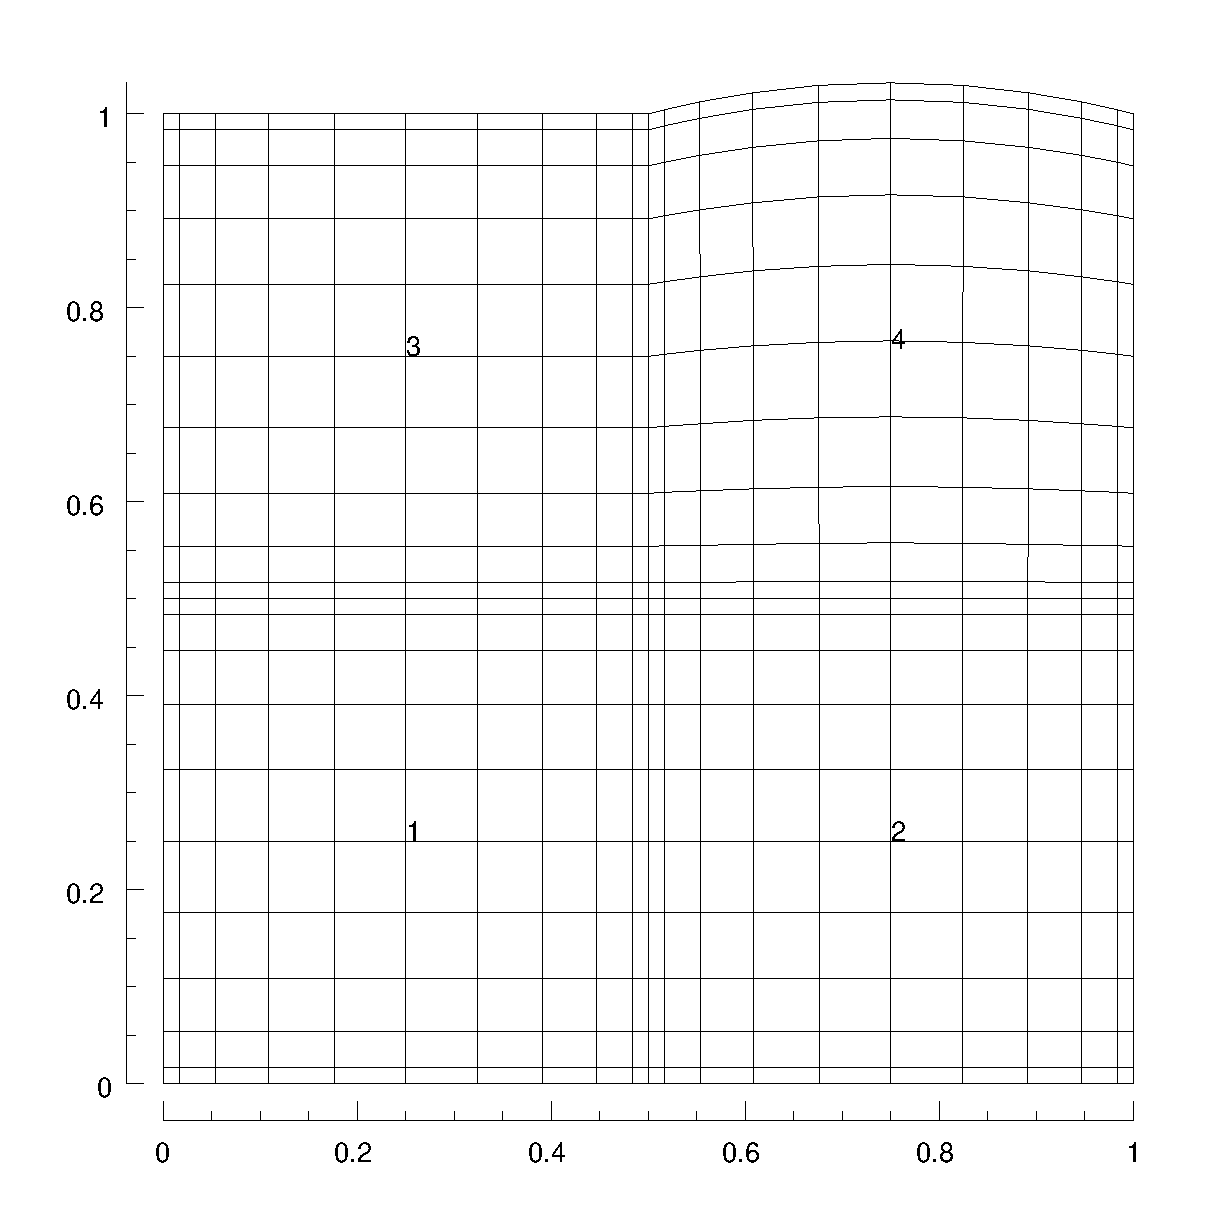
\includegraphics[width=0.5\textwidth]{laplace6mesh.eps}
\end{center}
\caption{
\label{lapcurve}
  The mesh corresponding to the \texttt{laplace6} session file.
}
\end{figure}

For the \texttt{SPLINE} type, the parameter supplies the name of an
ASCII file which contains a list of ($x$,\,$y$) coordinate pairs
(white-space delimited). Naturally, the list of points should be in
arc-length order. A single file can be used to supply the curved edges
for a set of element edges. The vertices of the relevant elements do
not have to lie exactly on the splined curve\,---\,if they do not,
those vertices get shifted to the intersection of the projection of
the straight line joining the original vertex position and its
neighbouring ``curve-normal' vertex, and the cubic spline joining the
points in the file. On the other hand, it is good practise to ensure
that the declared vertex locations lie close to the spline, and to
check the mesh that is produced: use \texttt{meshpr} to do this.

%----------------------------------------------------------------------------
\subsection{Boundary conditions}

The other new sections introduced in the session file for this example
(\texttt{GROUPS}, \texttt{BCS}) are used to impose boundary conditions
on the problem.  The \texttt{GROUPS} section associates a character
group tag (e.g. \verb+d+) with a string (e.g. \verb+value+), but note
that different groups can be associated with the same
string\footnote{This allows actions to be taken over a set of BCs
which share the same string.}.  Groups \verb+a+, \verb+b+ and \verb+c+
will be used to set natural (i.e. slope or Neumann), boundary
conditions, while group \verb+a+ will be used to impose an essential
or Dirichlet condition.

The \texttt{BCS} section is used to define the boundary conditions
which will be applied for each group.  For each group, after the
numeric tag (ignored) appears the character for that group, then the
number of BCs that will be applied: this corresponds to the number of
fields in the problem, in this case~1 (\verb+c+).  BCs can be only of
Dirichlet or Neumann type --- mixed BCs are not implemented yet.  So
in this case we will declare the BC types to be \verb+D+ ({\texttt
D}irichlet) for group \verb+d+ and \verb+N+ ({\texttt N}eumann) for
groups \verb+a+, \verb+b+ and \verb+c+.  On Neumann boundaries, the
value which must be supplied is the slope of the solution along the
outward normal to the solution domain.  Note the fact that the BCs can
be set using the function parser, using the built-in functions and
variables, also any symbols defined in the \texttt{TOKENS} section.
The BCs can be functions of time, \verb+t+, but in time-varying
problems the BCs are only set at the initial time, and not
subsequently re-parsed.

The BC groups are associated with element edges in the \texttt{SURFACES}
section, in a similar way to the use of periodic boundaries for the
\texttt{taylor2} problem, although the edges are set to be \verb+B+ (BC)
rather than \verb+P+ (periodic).

Periodic, Dirichlet and Neumann boundary conditions can be arbitrarily
mixed in a problem.  Dirichlet conditions over-ride Neumann ones where
they meet (say at the corner node of an element).

%----------------------------------------------------------------------------
\subsection{Running the codes}

We will run the solver and compare the computed solution to the
analytical solution.  We will select the iterative (PCG) solver using
the \verb+-i+ command-line option to \texttt{elliptic}, then check the 
result using \texttt{compare}.
{\small
\begin{verbatim}
karman[287] elliptic -i laplace6
-- Initializing solution with zero IC
   Start time       : 0
   Time step        : 0.01
   Number of steps  : 1
   End time         : 0.01
   Integration order: 2
karman[288] compare laplace6 laplace6.fld > /dev/null
Field 'c': norm_inf: 1.37112e-08
\end{verbatim}
}

Next try the direct solver (default):
{\small
\begin{verbatim}
karman[288] compare laplace6 laplace6.fld > /dev/null
Field 'c': norm_inf: 1.37112e-08
karman[289] elliptic laplace6
-- Initializing solution with zero IC
   Start time       : 0
   Time step        : 0.01
   Number of steps  : 1
   End time         : 0.01
   Integration order: 2
-- Building matrices for Fields "c"     [*]
karman[290] compare laplace6 laplace6.fld > /dev/null
Field 'c': norm_inf: 3.10862e-15
\end{verbatim}
}
\noindent
In this case the direct solver is more accurate, but this could be changed
by decreasing \verb+TOL_REL+ in the \texttt{TOKENS} section (and further
increasing \verb+STEP_MAX+, which has a default value of 500).

%============================================================================
\section{3D Kovasznay flow}

Here we will solve another viscous flow for which an analytical
solution exists, the Kovasznay flow (we will call the session file
\verb+kovas3+).  In the $x$--$y$ plane, this flow is
\begin{eqnarray}
        u &=& 1 - \exp(\lambda x)\cos(2\pi y)           \\
        v &=& \lambda/(2\pi)\exp(\lambda x)\sin(2\pi y) \\
        w &=& 0                                         \\
        p &=& (1 - \exp(\lambda x))/2   
\end{eqnarray}
where $\lambda = \Rey/2 - (0.25\Rey^2 + 4\pi^2)^{1/2}$.

Although the solution has only two velocity components, we will set up
and solve the problem in three dimensions, with a periodic length in
the~$z$ direction of~1.0 and 8~$z$ planes of data.  The length in the
$z$ direction is set within the code by the variable \verb+BETA+ where
$\beta=2\pi/L_z$.  The default value of \verb+BETA+ is 1, so we reset
this in the \texttt{TOKENS} section using the function parser.  The
exact velocity boundary conditions are supplied on at the left and
right edges of the domain, and periodic boundaries are used on the
upper and lower edges (the domain has $-0.5\le y\le0.5$).  Since the
flow evolves to a steady state, first order timestepping is employed
(\verb+N_TIME = 1+).

{\small
\begin{verbatim}
##############################################################################
# Kovasznay flow in the x--y plane has the exact solution
#
#       u = 1 - exp(lambda*x)*cos(2*PI*y)
#       v = lambda/(2*PI)*exp(lambda*x)*sin(2*PI*y)
#       w = 0
#       p = (1 - exp(lambda*x))/2
#
# where lambda = Re/2 - sqrt(0.25*Re*Re + 4*PI*PI).
#
# This 3D version uses symmetry planes on the upper and lower boundaries
# with flow in the x-y plane.
#
# Solution accuracy is independent of N_Z since all flow is in the x--y plane.

<USER>
        u = 1.0-exp(LAMBDA*x)*cos(TWOPI*y)
        v = LAMBDA/(TWOPI)*exp(LAMBDA*x)*sin(TWOPI*y)
        w = 0.0
        p = 0.5*(1.0-exp(LAMBDA*x))
</USER>

<FIELDS>
        u v w p
</FIELDS>

<TOKENS>
        N_Z    = 8
        N_TIME = 1
        N_P    = 8
        N_STEP = 500
        D_T    = 0.008
        Re     = 40.0
        KINVIS = 1.0/Re
        LAMBDA = Re/2.0-sqrt(0.25*Re*Re+4.0*PI*PI)
        Lz     = 1.0
        BETA   = TWOPI/Lz
</TOKENS>

<GROUPS NUMBER=1>
        1       v       velocity
</GROUPS>

<BCS NUMBER=1>
        1       v       4
                        <D> u = 1-exp(LAMBDA*x)*cos(2*PI*y)             </D>
                        <D> v = LAMBDA/(2*PI)*exp(LAMBDA*x)*sin(2*PI*y) </D>
                        <D> w = 0.0                                     </D>
                        <H> p                                           </H>
</BCS>

<NODES NUMBER=9>
        1      -0.5    -0.5     0.0
        2       0      -0.5     0.0
        3       1      -0.5     0.0
        4      -0.5     0       0.0
        5       0       0       0.0
        6       1       0       0.0
        7      -0.5     0.5     0.0
        8       0       0.5     0.0
        9       1       0.5     0.0
</NODES>

<ELEMENTS NUMBER=4>
        1 <Q> 1 2 5 4 </Q>
        2 <Q> 2 3 6 5 </Q>
        3 <Q> 4 5 8 7 </Q>
        4 <Q> 5 6 9 8 </Q>
</ELEMENTS>

<SURFACES NUMBER=6>
        1       1       1       <P>     3       3       </P>
        2       2       1       <P>     4       3       </P>
        3       2       2       <B>     v               </B>
        4       4       2       <B>     v               </B>
        5       3       4       <B>     v               </B>
        6       1       4       <B>     v               </B>
</SURFACES>
\end{verbatim}
}

%----------------------------------------------------------------------------
\subsection{`High-order' pressure boundary condition}

Note that there is only one boundary group, and four boundary
conditions must be set, corresponding to the four fields \verb+u+,
\verb+v+, \verb+w+ and \verb+p+.  A new feature is a pressure BC of
type \verb+H+, which is an internally-computed Neumann boundary
condition, (a \verb+H+igh-order pressure BC) as described in
\citet{kio91}.  This is the kind of pressure BC that is supplied at
all places except on outflow boundaries.  The pressure BC is computed
internally, so no value is required (if given, it will be ignored).

%----------------------------------------------------------------------------
\subsection{Running the codes}

After running \verb+dns+, we confirm there is only a single dump in the
field file \verb+kovas3.fld+, then run compare in order to examine the
error norms for the solution.  Following that we prepare input for
TECPLOT, projecting the interpolation to a $20\times20$ grid in each
element.  A view of the result can be seen in figure~\ref{kov3soln}.
{\small
\begin{verbatim}
karman[25] convert kovas3.fld | grep -i session
kovas3                    Session
karman[26] compare kovas3 kovas3.fld > /dev/null
Field 'u': norm_inf: 5.70744e-05
Field 'v': norm_inf: 3.04095e-05
Field 'w': norm_inf: 0
Field 'p': norm_inf: 0.928545
karman[27] meshpr kovas3 | sem2tec -n20 kovas3.fld
\end{verbatim}
}
\begin{figure}
\begin{center}
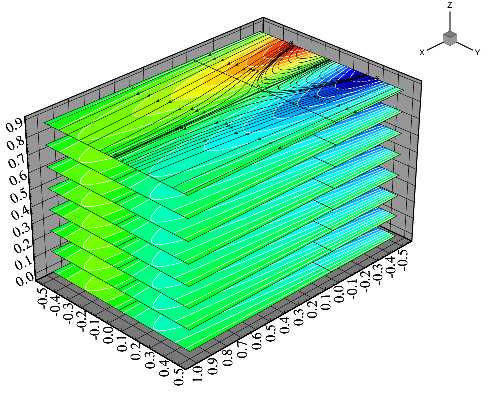
\includegraphics[width=0.75\textwidth]{kovas3_bitmap.eps}
\end{center}
\caption{
\label{kov3soln}
  Solution to the \texttt{kovas3} problem, visualized using TECPLOT.
  The plot shows contours of $v$ velocity component and streamlines.
  }
\end{figure}

%============================================================================
\section{Vortex breakdown\,---\,a cylindrical problem}

Here we will examine a problem which uses the cylindrical coordinate
option of \verb+dns+.  The physical situation is a cylindrical cavity,
$H/R=2.5$ with the flow driven by a spinning lid at one end.  At the
Reynolds number we'll use, $\Rey=\Omega R^2/\nu=2119$, a vortex
breakdown is known to occur.  The flow in this case is invariant in
the azimuthal direction, so we will solve with only two azimuthal
planes: in fact in the Fourier decomposition, the second plane will
correspond to the spatial Nyquist frequency and the code will set it
to zero with no temporal evolution.  There must be at least two
azimuthal planes in order to to have three velocity components however
it would be possible to write a code which solved for three velocity
components in two dimensions.  In the cylindrical code, the order of
spatial directions and velocity components is $z$, $r$, $\theta$.
Note for a full circle in the azimuthal direction, \texttt{BETA =
1.0}, (which is the default value).

{\small
\begin{verbatim}
#############################################################################
# 15 element driven cavity flow.

<FIELDS>
        u v w p
</FIELDS>

<TOKENS>
        CYLINDRICAL = 1
        N_Z         = 2
        BETA        = 1.0
        N_TIME      = 2
        N_P         = 11
        N_STEP      = 100000
        D_T         = 0.01
        KINVIS      = 0.000472
        OMEGA       = 1.0
        TOL_REL     = 1e-12
</TOKENS>

<GROUPS NUMBER=3>
        1       v       velocity
        2       w       wall
        3       a       axis
</GROUPS>

<BCS NUMBER=3>
        1       v       4
                        <D>     u = 0           </D>
                        <D>     v = 0           </D>
                        <D>     w = OMEGA*y     </D>
                        <H>     p               </H>
        2       w       4
                        <D>     u = 0           </D>
                        <D>     v = 0           </D>
                        <D>     w = 0           </D>
                        <H>     p               </H>
        3       a       4
                        <A>     u               </A>
                        <A>     v               </A>
                        <A>     w               </A>
                        <A>     p               </A>
</BCS>

<NODES NUMBER=24>
        1       0       0       0
        2       0.4     0       0
        3       0.8     0       0
        4       1.5     0       0
        5       2.4     0       0
        6       2.5     0       0
        7       0       0.15    0
        8       0.4     0.15    0
        9       0.8     0.15    0
        10      1.5     0.15    0
        11      2.4     0.15    0
        12      2.5     0.15    0
        13      0       0.75    0
        14      0.4     0.75    0
        15      0.8     0.75    0
        16      1.5     0.818   0
        17      2.4     0.9     0
        18      2.5     0.9     0
        19      0       1       0
        20      0.4     1       0
        21      0.8     1       0
        22      1.5     1       0
        23      2.4     1       0
        24      2.5     1       0
</NODES>

<ELEMENTS NUMBER=15>
        1       <Q>      1  2  8  7     </Q>
        2       <Q>      2  3  9  8     </Q>
        3       <Q>      3  4 10  9     </Q>
        4       <Q>      4  5 11 10     </Q>
        5       <Q>      5  6 12 11     </Q>
        6       <Q>      7  8 14 13     </Q>
        7       <Q>      8  9 15 14     </Q>
        8       <Q>      9 10 16 15     </Q>
        9       <Q>     10 11 17 16     </Q>
        10      <Q>     11 12 18 17     </Q>
        11      <Q>     13 14 20 19     </Q>
        12      <Q>     14 15 21 20     </Q>
        13      <Q>     15 16 22 21     </Q>
        14      <Q>     16 17 23 22     </Q>
        15      <Q>     17 18 24 23     </Q>
</ELEMENTS>

<SURFACES NUMBER=16>
        1       1       1       <B>     a       </B>
        2       2       1       <B>     a       </B>
        3       3       1       <B>     a       </B>
        4       4       1       <B>     a       </B>
        5       5       1       <B>     a       </B>
        6       5       2       <B>     v       </B>
        7       10      2       <B>     v       </B>
        8       15      2       <B>     v       </B>
        9       15      3       <B>     w       </B>
        10      14      3       <B>     w       </B>
        11      13      3       <B>     w       </B>
        12      12      3       <B>     w       </B>
        13      11      3       <B>     w       </B>
        14      11      4       <B>     w       </B>
        15      6       4       <B>     w       </B>
        16      1       4       <B>     w       </B>
</SURFACES>
\end{verbatim}
}

The mesh for the problem is shown in figure~\ref{vb1msh}, and the
velocity field is shown compared to an experimental streakline flow
visualisation on the front cover of this document.
\begin{figure}
\begin{center}
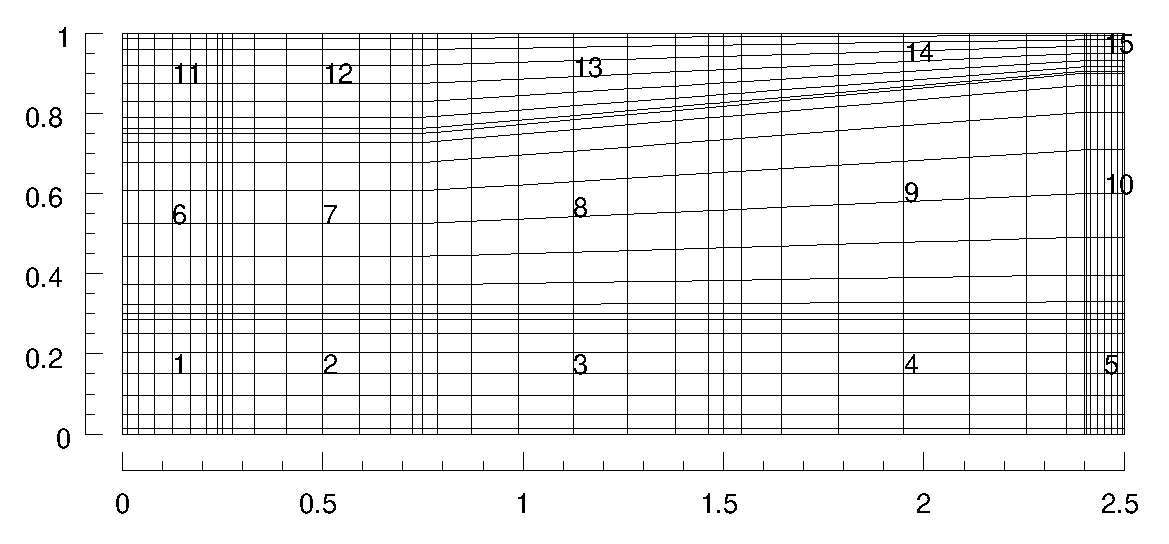
\includegraphics[width=0.75\textwidth]{vb1mesh.eps}
\end{center}
\caption{
\label{vb1msh}
  Mesh for the vortex breakdown problem.  The spinning lid is at right.
  }
\end{figure}

%----------------------------------------------------------------------------
\subsection{BCs for cylindrical coordinates}

A new feature here is the use of BCs of type \verb+A+ on the axis of
the flow.  Internally, the code sets the BC there either as zero
essential or zero natural, depending on the physical variable and the
Fourier mode.  Owing to the coupling scheme used in the code
\cite{blsh04}, the boundary conditions for the radial and azimuthal
velocities \verb+v+ and \verb+w+ must be of the same type within each
group.  A further restriction is that the group to which the axis
belongs must have name \verb+axis+.

%%%%%%%%%%%%%%%%%%%%%%%%%%%%%%%%%%%%%%%%%%%%%%%%%%%%%%%%%%%%%%%%%%%%%%%%%%%%%%
\chapter{Extra controls}

This chapter describes some additional features that are implemented
within the Navier--Stokes solver \verb+dns+ to control execution and
output.

%=============================================================================
\section{Checkpointing}

By default, intermediate solutions are appended to \verb+session.fld+
every \verb+IO_FLD+ steps (default value \verb+IO_FLD = 500+).  For
lengthy or 3D simulations, \verb+session.fld+ can quickly grow to an
unreasonable size.  Controlling this by setting \verb+IO_FLD = N_STEPS+
can be risky, as the simulation could become unstable or be terminated
before ending as expected.  A better approach (unless the intermediate
fields are desired for postprocessing) is to use checkpointing.  With
\verb+CHKPOINT = 1+, intermediate field dumps are written to
\verb+session.chk+, rotating to \verb+session.chk.bak+ every
\verb+IO_FLD+ steps, until the end of the simulation, when
\verb+session.fld+ is written.  A command line option (\verb+dns -chk+)
can also be used to select checkpointing, but this is
over-ridden by whatever is set in the \verb+session+ file.

%=============================================================================
\section{Iterative solution}

Two matrix solution methods are implemented for Helmholtz problems
associated with the pressure and viscous substeps of the time
splitting.  By default, direct Schur-complement solutions are used.
The associated global matrices can consume quite large amounts of
memory, typically much more than is required for storage of the
associated field variable.  Iterative (PCG) solution can also be
selected, and this has the advantage that since it is matrix-free, no
global matrices are required, however, solution may be slower than for
the direct solver (depending on the condition number of the global
matrix problem).

The token that controls the selection of solution method is
\verb+ITERATIVE+.  For \verb+dns+, PCG solution can be selected for
the viscous substep of the solution (\verb+ITERATIVE = 1+), or for
both viscous and pressure substeps (\verb+ITERATIVE = 2+).  The same
functions can be selected by command-line options (\verb+dns -i+
$\equiv$ \verb+ITERATIVE = 1+, while \verb+dns -ii+ $\equiv$
\verb+ITERATIVE = 2+), but note that these options are overridden by
whatever tokens are set in the \verb+session+ file (the default value
is \verb+ITERATIVE = 0+).

Iterative solution is most useful for the viscous substep,
particularly when the Reynolds number is high, since this decreases
the condition number of the associated global matrices.  In fact,
iterative solutions for the viscous substep can execute faster than
direct solutions at high Reynolds number, although this is platform
dependent.  Since the global pressure matrices have higher condition
numbers, particularly for low Fourier modes, iterative solution for
the pressure substep is only of any practical use when memory at a
premium.

%=============================================================================
\section{Wall fluxes}

A file called \verb+session.flx+ is used to store the integral over
the \verb+wall+ group boundaries of viscous and pressure stresses
(i.e.\ lift and drag forces).  Output is done every \verb+IO_HIS+
steps.  For each direction ($x$, $y$, $z$), the outputs are in turn
the pressure, viscous, and total force per unit length.  In 2D the
$z$-components are always zero, while in 3D the $z$-component pressure
force is always zero, owing to the fact that the geometry is invariant
in that direction.  For cylindrical geometries, the output values are
forces per radian (in the $x$ and $y$ directions) and torque per
radian (in the $z$ direction) rather than forces per unit length.

%=============================================================================
\section{Wall tractions}

If the token \verb+IO_WSS+ is set to a non-zero value then the normal
and the single (2D) or two (3D) components of tangential boundary
traction are computed on the \verb+wall+ group, and output every
\verb+IO_WSS+ steps in the file \verb+session.wss+.  This is a binary
file with structure similar to a field dump.  The utility
\verb+wallmesh+ is used to extract the corresponding mesh points
along the walls.

%=============================================================================
\section{Modal energies}

For 3D simulations (\verb+N_Z > 2+), a file of modal energies,
\verb+session.mdl+, is produced.  This provides valuable diagnostic
information for turbulent flow simulations.  For each active Fourier
mode $k$ in the simulation, the value output every \verb+IO_HIS+ steps
is 
\[
E_k =
\frac{1}{2A}\int_\Omega
\hat{\bs{u}}_k^\ast\cdot\hat{\bs{u}}_k \,{\rm d}\Omega,
\]
where $A$ is the area of the 2D domain~$\Omega$.  Each line of the
file contains the time $t$, mode number $k$ and $E_k$.

%=============================================================================
\section{History points}

History points are used to record solution variables at fixed spatial
locations as the simulation proceeds.  The locations need not
correspond to grid points, as data are interpolated onto the given
spatial locations using the elemental basis functions.  Locations of
history points are declared in the \verb+session+ file as follows:
\begin{verbatim}
<HISTORY NUMBER=1>
#       tag     x       y       z 
        1       0       0       0
</HISTORY>
\end{verbatim}

A file called \verb+session.his+ is produced as output.  Each line of
the file contains the step number, the time, the history point tag
number, followed by values for each of the solution variables.  The
step interval at which history point information is dumped to file is
controlled by the \verb+IO_HIS+ token; the default value is
\verb+IO_HIS = 10+.

%=============================================================================
\section{Averaging}

Set \verb+AVERAGE = 1+ in the tokens section to get averages of field
variables left in files \verb+session.ave+ and \verb+session.avg+
(which are analogous to \verb+session.chk+ and \verb+session.fld+, but
\verb+session.ave.bak+ is not produced).  Averages are updated
every \verb+IO_HIS+ steps, and dumped every \verb+IO_FLD+ steps.
Restarts are made by reading \verb+session.avg+ if it exists.

Setting \verb+AVERAGE = 2+ will accumlate averages for Reynolds
stresses as well, with reserved names \verb+ABCDEF+, corresponding to
products
\begin{verbatim}
uu uv uw     A  B  D
   vv vw  =     C  E
      ww           F
\end{verbatim}
The hierarchy is named this way to allow accumlation of products in 2D
as well as 3D (for 2D you get only \verb+ABC+).  In order to actually
compute the Reynolds stresses from the accumulated products you need
to run the \verb+rstress+ utility, which subtracts the products of the
means from the means of the products:
\begin{verbatim}
rstress session.avg > reynolds-stress.fld
\end{verbatim}
An alternative function of \verb+rstress+ is to subtract one field
file from another:
\begin{verbatim}
rstress good.fld test.fld | convert | diff
\end{verbatim}

Setting \verb+AVERAGE = 3+ will accumlate sums of additional products
for computation of terms in the energy transport equation. You will
then need to use the \verb+eneq+ utility to actually compute the
terms. Presently this part of the code is only written for Cartesian
coordinates.


%=============================================================================
\section{Particle tracking}

The code allows for tracking of massless particles, but this only
works correctly for non-concurrent execution at present.  Tracking is
quite an expensive operation, since Newton--Raphson iteration is used
to relocate particles within each element at every timestep.

The application looks for a file called \verb+session.par+.  Each line
of this file is of form
\begin{verbatim}
#     tag  time  ctime  x     y      z
      1    0.0   0.0    1.0   10.0   0.5.
\end{verbatim}
The \verb+time+ value is the integration time, while \verb+ctime+
records the time at which integration was initialised.

Output is of the same form, and is called \verb+session.trk+.  The use
of separate files, rather than by declaration in the session file, is
intended so that \verb+session.trk+ files can be moved to
\verb+session.par+ files for restarting.  Particles that aren't in the
domain at startup, or leave the domain during execution, are deleted.

Setting \verb+SPAWN = 1+, re-initiates extra particles at the original
positions every timestep.  With spawning, particle tracking can
quickly grow to become the most time-consuming part of execution.

%%%%%%%%%%%%%%%%%%%%%%%%%%%%%%%%%%%%%%%%%%%%%%%%%%%%%%%%%%%%%%%%%%%%%%%%%%%%%%
\chapter{Compilation of specialised executables}

The special compilations below can be combined.

%=============================================================================
\section{Concurrent execution}

The code supports concurrent execution for 3D simulations, with MPI
used as the message-passing kernel. Compile using \verb+make MPI=1+ to
produce \verb+dns_mp+. (You will also need to compile in the
appropriate message-passing routines in compiling \verb+femlib+, for
which change to the \verb+femlib+ directory, then do
\verb+make clean; make MPI=1; make install MPI=1+.)  Nonlinear terms
are not dealiased when running in parallel, but are dealiased in the
Fourier direction when running on one process, or running the serial
code. To get a serial code that does not perform dealiasing on Fourier
terms (e.g.\ for cross-checking), compile the serial code using
\verb+make ALIAS=1+ to produce \verb+dns_alias+ (in which case make
sure you delete \verb+nonlinear.o+ first).

%=============================================================================
\section{Time-varying boundary conditions}

By default, the velocity boundary conditions are frozen for the time
corresponding to the initial conditions. If you compile with
\verb+make TBCS=1+ you will generate \verb+dns_tbcs+ in which the
\emph{zeroth Fourier mode's} (2D) velocity boundary conditions are
re-evaluated every time step. Usually one only wants to vary the 2D
boundary conditions. NB: make sure you delete \verb+integrate.o+
first.

%=============================================================================
\section{Convective advection terms}

By default, the code computes the nonlinear advection terms in
skew-symmetric form $0.5(\bm{\nabla\cdot u u}+\bm{u\cdot\nabla u})$,
as this seems to be the most robust at high Reynolds numbers. However,
it is also comparatively costly. If you want to compile a code with
only the standard convective terms $\bm{u\cdot\nabla u}$, compile with
\verb+make CONV=1+ to produce \verb+dns_conv+.  NB: make sure you
delete \verb+nonlinear.o+ first.

%=============================================================================
\section{Stokes solver}

To produce an unsteady Stokes solver (i.e.\ \verb+dns+ without
nonlinear terms included), compile using \verb+make STOKES=1+, to
produce the executable \verb+dns_stokes+.  NB: make sure you delete
\verb+nonlinear.o+ first.

%%%%%%%%%%%%%%%%%%%%%%%%%%%%%%%%%%%%%%%%%%%%%%%%%%%%%%%%%%%%%%%%%%%%%%%%%%%%%

\bibliographystyle{dcu}
\bibliography{userguide}

%%%%%%%%%%%%%%%%%%%%%%%%%%%%%%%%%%%%%%%%%%%%%%%%%%%%%%%%%%%%%%%%%%%%%%%%%%%%%
\end{document}
